\subsubsection{Paketinis gradientinis nusileidimas}
\label{subsubsec:klasifikavimo_tikslumas_paketinis_gradientinis_nusileidimas}

Klasifikavimo tikslumas sparčiai auga pirmųjų epochų metu ir stabilizuojasi apie $97\ \%$ mokymo duomenims bei $98{,}2\ \%$ validavimo duomenims (žr.~\ref{fig:accuracy_bgd} pav.).

\begin{figure}[H]
    \centering
    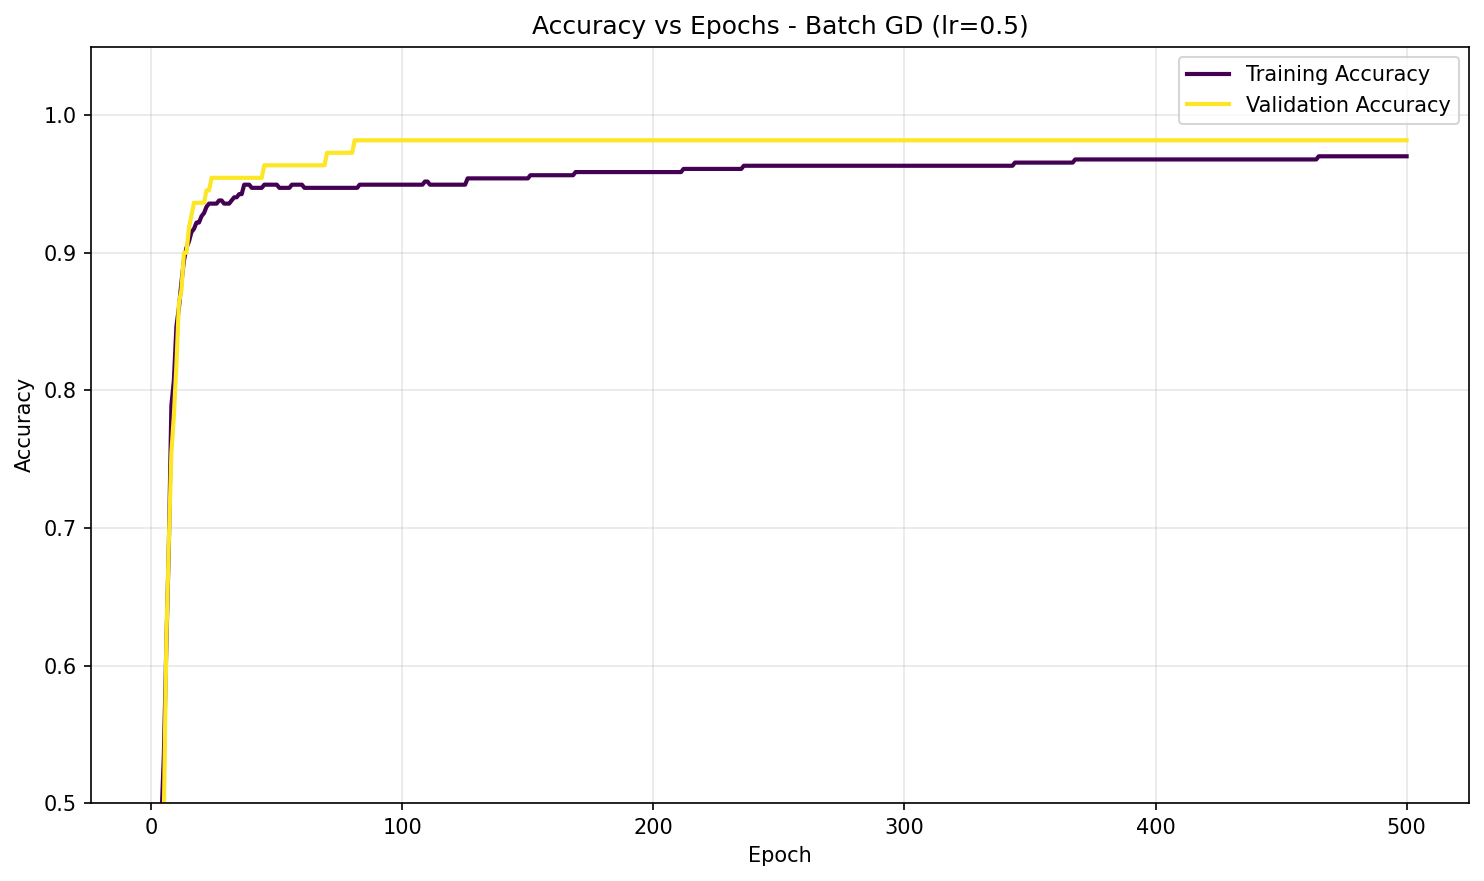
\includegraphics[width=0.85\linewidth]{2Lab/visualizations/accuracy_bgd.png}
    \caption{Klasifikavimo tikslumo priklausomybė nuo epochų (paketinis GN, $\eta = 0{,}5$)}
    \label{fig:accuracy_bgd}
\end{figure}